%===================================== CHAP 5 =================================

\chapter{Results}
\label{ch:results}

The results from performing the test cases described in section \ref{Method} are presented in this chapter. Section \ref{sec:CASE1_r}, \ref{sec:CASE2_r} and \ref{sec:CASE3_r}, gives the results from test case 1, 2 and 3 respectively. Plots of errors and visualizations of the estimates are given. 

\section{CASE 1}
\label{sec:CASE1_r}
50 Newton iterations for a constant generative weight, $w_{21} = 0.7$, for $T=1000$ and initial guess $w_{12}^{(0)} = 2$ were performed according to the description in section \ref{sec:CASE1}. The estimated weigh after the last iteration was $w_{21}^{(50)}=0.679$. The left plot in figure \ref{fig:Newton} illustrates the likelihood function, and the points for the initial guess, and the estimated weight after 1, 2, 3 and 50 iterations. The right plot shows the estimated weigh at every iteration.

%The learning was on purpose set slower, in order to give a better visual representation. 


\begin{figure}[hbt!]
\caption{(Left) Log-likelihood with starting point, 1st, 2nd, 3rd and 50th iteration marked. (Right) Estimated weight for each iteration.}
\label{fig:Newton}
    \centering
    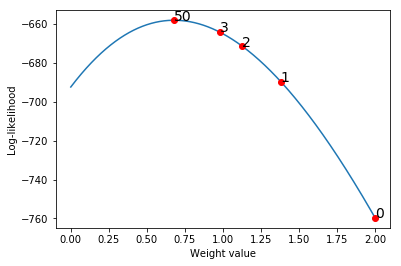
\includegraphics[scale=0.40]{Step_1.png}
    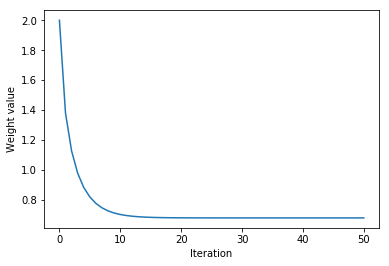
\includegraphics[scale=0.40]{fig/Step_1_it.png}
\end{figure}

One can conclude that the algorithm converges by visual inspection of the plots. Also, the estimated weight in the five last iterations are equal up to seven decimals. To arrive at two decimals precision it took 18 iterations. However, the inferred weight and the generative weight differ by $w_{21} - w_{21}^{(50)} = 0.021$. This difference is not due to any failure of the algorithm to find the maximum likelihood, but rather due to the fact that for a finite data sample the actual maximum likelihood value in the data might differ from the underlying parameter that generated them. This will improve as the size of the data set increases. To illustrate this point, the algorithm was run 1000 times each for $T \in \{ 100,1000,10000\}$. Histograms for the maximum likelihood estimates is shown in figure \ref{fig:ML_hist}. Although in all cases the estimates are centered around the true value,  the variance in the estimates are smaller for a bigger sample. 

\begin{figure}[hbt!]
    \centering
    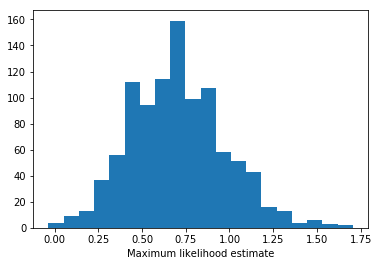
\includegraphics[scale = 0.40]{fig/ML_100.png}
    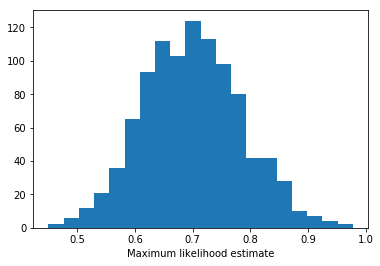
\includegraphics[scale = 0.40]{fig/ML_1000.png}
    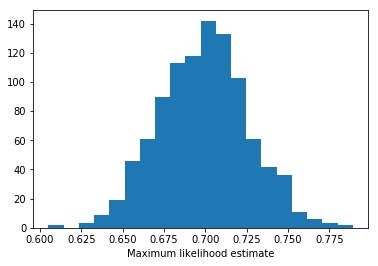
\includegraphics[scale = 0.40]{fig/ML_10000.png}
    \caption{Histograms of estimated weighs from 1000 replicates with 100 (top left), 1000 (top right) and 10000 (bottom) time steps}
    \label{fig:ML_hist}
\end{figure}

\section{CASE 2}
\label{sec:CASE2_r}
The procedure described in section \ref{sec:CASE2}, and summarized in algorithm \ref{alg:M-H} was performed with 3000 iterations, for various number of spike trains, $ \{1,10,100,1000,10000 \}$. Firstly, the initial guess was set equal to the generative weights, namely $\bf w_{12}^{(0)} = \bf w_{12}$. This gives a starting error of zero. Figure \ref{fig:Case2_1} shows an example of normalized root mean squared errors over iterations for the different number of trials. Here the generative weight trajectory, as exemplified in figure \ref{fig:Generative} was the same for all the instances, and the initial guess was set to be the true weights. 


\begin{figure}[hbt!]
\caption{Normalized root MSE over iterations for various number of trials. One example of the method in case 2 when starting from the correct weights}
\label{fig:Case2_1}
    \centering
    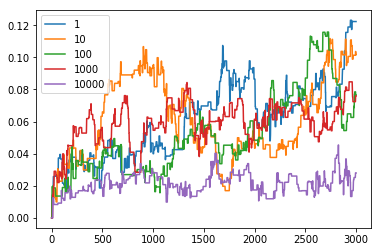
\includegraphics[scale=0.6]{MSE3.png}
\end{figure}

This shows that for the lower number of trials the estimation jumps around, whereas for 10000 trials it is more stable.

This procedure was repeated 100 times for each number of trials. The underlying weights were now drawn new for each replicate. Figure \ref{fig:case2_avg} shows the mean of the rnMSE values at each iteration, with variance bars around it. 

\begin{figure}[hbt!]
\caption{Average rnMSE with variance bars of 100 replicates for each number of trials. Initial guess set to the generative weights.}
\label{fig:case2_avg}
    \centering
    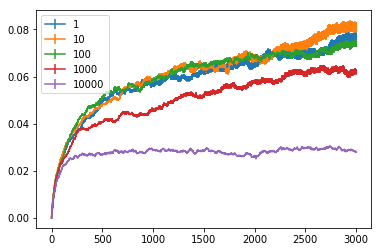
\includegraphics[scale=0.6]{Mean_plot_std.png}
\end{figure}

%\begin{figure}[hbt!]
    %\centering
    %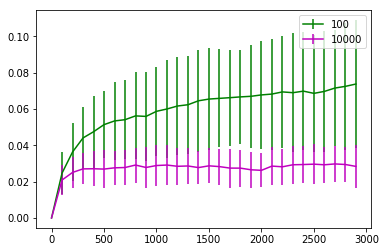
\includegraphics[scale=0.8]{Std_every100.png}
%\end{figure}


Next, the initial guess for the iterations is set to be a random walk around 1. Figure \ref{fig:MSE2} shows the corresponding mean rnMSE of 100 replicates for each number of trials, with variance bars. 

%\begin{figure}[hbt!]
    %\centering
    %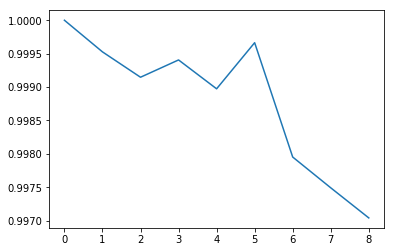
\includegraphics[scale=0.8]{Start_it_1000.png}
%\end{figure}


\begin{figure}[hbt!]
\caption{Average rnMSE with variance bars of 100 replicates for each number of trials. Initial guess set to random walk around 1}
\label{fig:MSE2}
    \centering
    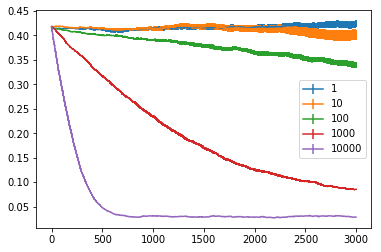
\includegraphics[scale=0.6]{MSE_starting_away.png}
\end{figure}

As clear from the plots, the relaxation time for the learning is dependent on the number of trials. For initial guess equal to the generative weights, saturation happens after around 300 iterations for 10000 trials, and around 2500 iterations for 1000 trials. For smaller number of trials the solution is still moving away from the solution after 3000 iterations. Figure \ref{fig:MSE2} show that also for 100 trials there is a slow movement in the correct direction. The figures also show that the solution is more stable for the higher number of trials, since the variance bars are thinner.  

To visualize what is happening during the course of the iterations figure \ref{fig:trajectories} displays the how the last accepted weight trajectory to the sample after 100,200,300,400,500 and 1000 iterations looks like, for initial guess a random walk around 1 and 10000 trials. 

Figure \ref{fig:trajectories} shows that the weight trajectory shifts rigidly across iterations towards the generative value, and eventually ends up relatively close to the true weights. This is enforced by the prior distribution, which demands a continuity in time. 

\begin{figure}[P]
\caption{Plots of the true weights (blue), the initial guess (orange), and the inferred weights after 100, 200, 300, 400, 500 and 1000 iterations (green)}
\label{fig:trajectories}
    \centering
    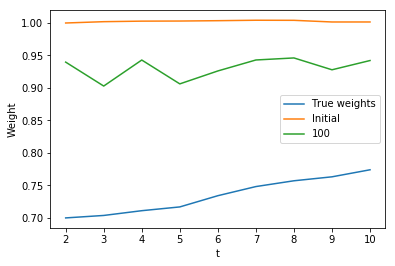
\includegraphics[scale=0.4]{fig/10000_100.png}
    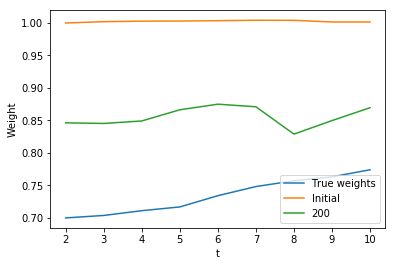
\includegraphics[scale = 0.4]{fig/10000_200.png}\\
    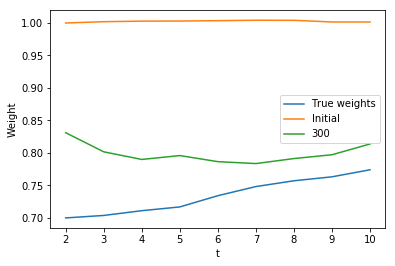
\includegraphics[scale = 0.4]{fig/10000_300.png}
    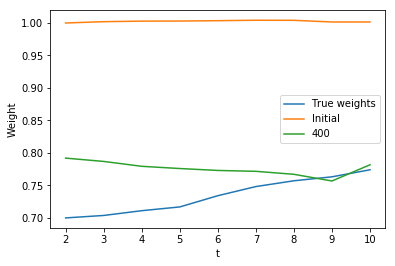
\includegraphics[scale = 0.4]{fig/10000_400.png}\\
    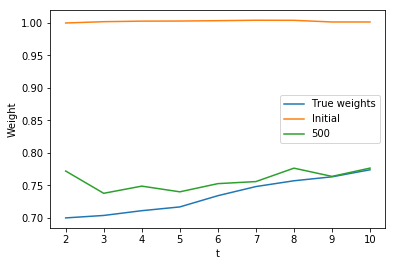
\includegraphics[scale = 0.4]{fig/10000_500.png}
    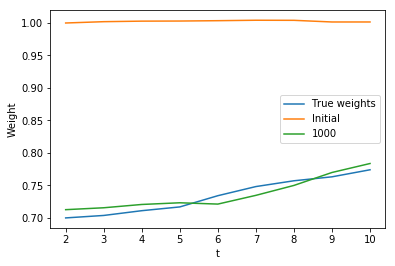
\includegraphics[scale = 0.4]{fig/10000_1000.png}
\end{figure}

It was also investigated what happens during the iterations for a lower number of trials. For exemplification, with 10 trials various values for the prior variance was tried to see if the results could be improved. All variants gave fluctuating error over iterations, except when the prior was set so strict that no steps were accepted. Figure \ref{fig:10st} illustrates the weight trajectory after 10000 iterations for prior variances in $\{ 0.1, 0.01, 0.001, 0.0001, 0.00001\}$. 10000 iterations was chosen to be sure that if any convergence took place, this would be shown. 

\begin{figure}[P]
\caption{Plots of the true weights (blue), the initial guess (orange), and the inferred weights after 10000 iterations with 10 spike trains, and a prior variance of 0.1, 0.01, 0.001, 0.0001 and 0.00001}
\label{fig:10st}
    \centering
    \includegraphics[scale=0.4]{{10st_0.1prior}.png}
    \includegraphics[scale = 0.4]{{10st_0.01prior}.png}\\
    \includegraphics[scale = 0.4]{{10st_0.001prior}.png}
    \includegraphics[scale = 0.4]{{10st_0.0001prior}.png}\\
    \includegraphics[scale = 0.4]{{10st_0.00001prior}.png}
\end{figure}

As seen the starting trajectory used here is quite flat. One could think that this could stop the trajectory from moving away from its starting position, since it is already too good in terms of the prior. Therefore it was also tried a much more variate starting point, and a strict prior variance of 0.00001, to see the result then. The weight after 10000 iterations for this variant is shown in figure \ref{fig:10st2}.

\begin{figure}
    \centering
    \includegraphics[scale=0.6]{{10st_0.00001prior_1starting}.png}
    \caption{Plots of the true weights (blue), the initial guess (orange), and the inferred weights after 10000 iterations with 10 spike trains, and a prior variance of 0.00001. Initial weight trajectory for the iterations were drawn with }
    \label{fig:10st2}
\end{figure}


\section{CASE 3}
\label{sec:CASE3_r}
First the variant where the weight for all time steps are drawn individually was performed. This was tried with various values for the variance in the prior and proposal distribution. For a low value of the prior variance compared to the proposal variance, no new weight trajectories were accepted in the algorithm, so the estimation just stays where it starts. If the relative variance is large enough for weight trajectories to be accepted, it does not move towards the correct solution, and the error increases with iteration. One example of the generative, initial and inferred weights after 3000 iterations is shown in figure \ref{fig:400_weights}. 


\begin{figure}
    \caption{True weights (orange), initial guess (green) and inferred weights (blue) after 3000 iterations}
    \label{fig:400_weights}
    \centering
    \includegraphics[scale=0.6]{fig/{Result_0.08}.png}
\end{figure}


Next, the same procedure was performed with dividing the time line into windows, and assuming constant weights within the windows. The initial guess was set to a random walk around 1. The result for dividing 300 seconds into 10 windows, and performing 3000 iterations is shown in figure \ref{fig:10bins}, with prior and proposal variance equal to 0.01, 0.005 and 0.0005.


\begin{figure}[hbt!]
\caption{True weights (orange), initial guess (green) and inferred weights (blue) for 10 bins and 3000 iterations. The prior and proposal distribution was 0.01 (top left), 0.005 (top right) and 0.0005 (bottom)}
\label{fig:10bins}
    \centering
    \includegraphics[scale=0.45]{fig/{10bins_0.01_0.01_s}.png}
    \includegraphics[scale=0.45]{fig/{10bins_0.005_0.005_s}.png}\\
    \includegraphics[scale=0.45]{fig/{10bins_0.0005_0.0005}.png}
\end{figure}

Figure \ref{fig:10bins} shows that $0.01$ and $0.005$ gives a reasonable result, whereas $0.0005$ forces a time continuity that is too strict to properly capture the dynamics.

This was done for 1, 5, 10 and 20 number of windows, with 30 replicates for each. The mean of the rnMSE with variance bars for these are presented in figure \ref{fig:MSE_bins}. Here the prior and proposal variance used was 0.005, which was chosen as it gave reasonable results. 

\begin{figure}[hbt!]
\caption{}
\label{fig:MSE_bins}
    \centering
    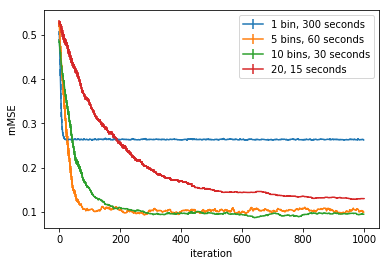
\includegraphics[scale=0.6]{fig/MSE_bins.png}
\end{figure}


It is clear from figure \ref{fig:MSE_bins} that there is a trade-off between the constraint imposed by the time windows and the ability to update towards likelier parameters. With 10 windows the number of weights to infer is almost the same as in test case 2, where there was 9. However, it is interesting to note saturation is reached faster. The value of the rnMSE is bigger than in case 2. This is reasonable, as we set a constant weight in each window when the true weight is varying over the window. 

\begin{figure}[hbt!]
\caption{Plot of average rnMSE of 20 replicates with 10 windows for prior variances equal to 1, 0.1, 0.02 and 0.005}
\label{fig:prior_variance}
    \centering
    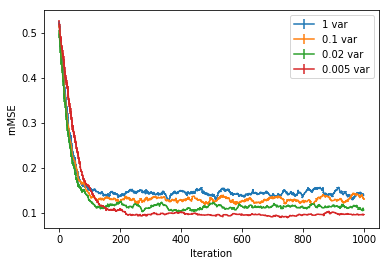
\includegraphics[scale=0.6]{fig/Prior_variance_plot.png}
\end{figure}


\cleardoublepage